\chapter{Project Execution}
\label{chap:execution}


\section{Introduction}
The main activity of this project was the development of a mobile app that can usefully analyse intermediate climbers' technique and then provide them with various data whilst they climbing, whether it be for training or fun.
To do this, I performed a User-Centred iterative design process, with four large main iterations, and many smaller ones to guide along the way.


\subsection{User-Centred Iterative Design}
Throughout the execution of the development of this project, I followed the guidelines of both the Iterative Design and User-Centred Design methodologies.

\subsubsection{Iterative Design}
Iterative Design is a methodology where a cyclic process of prototypes, tests, analysis, and refinements of a product are made.
See Figure~\ref{fig:iter}.


\begin{figure}[h]
\centering
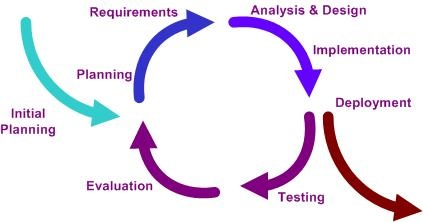
\includegraphics[width=10cm]{imgs/iterativeloop}
\caption{Diagram of the Iterative Development Model. \newline \textit{\small Westerhoff [Public domain], via Wikimedia Commons}}
\label{fig:iter}
\end{figure}

% \begin{figure}[h]
% \centering
% 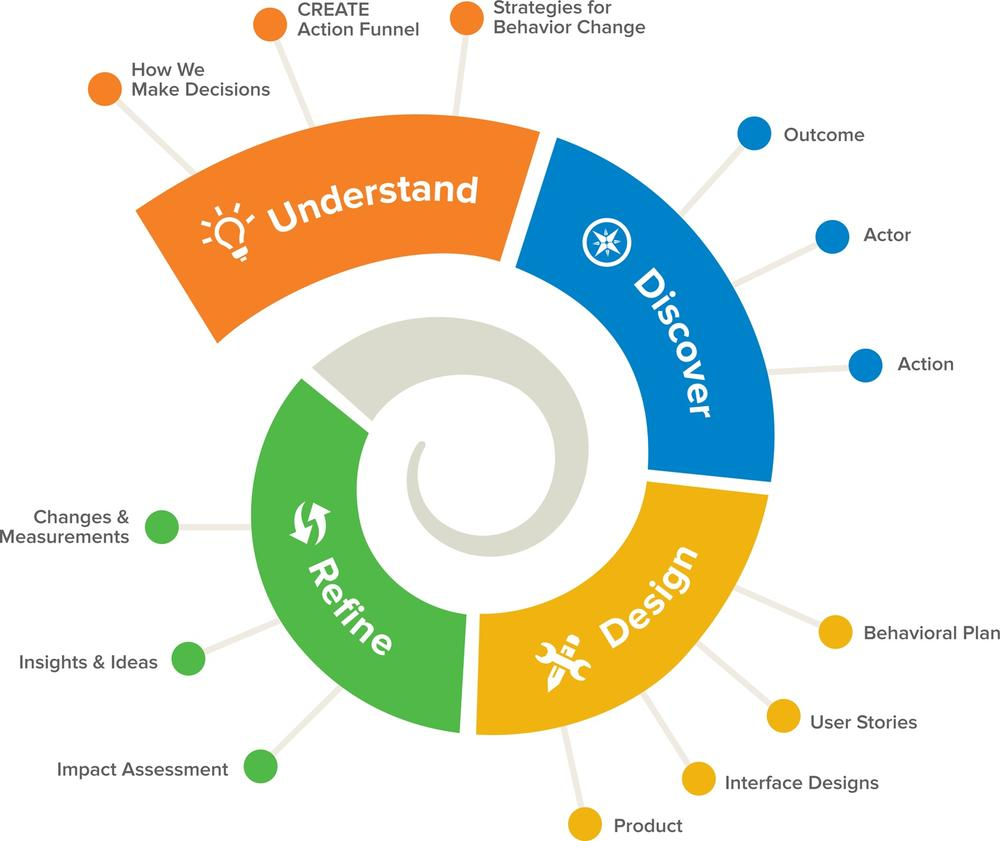
\includegraphics[width=10cm]{imgs/itrativespiral}
% \caption{Spiral Diagram of the Iterative Development Model.  \textit{\small Fig. 23 from Designing for Behavior Change
% by Stephen Wendel}}
% \label{fig:iter}
% \end{figure}

After some initial plans have been made, a set of requirements are laid out, then some very basic form of the product is implemented, before being tested to gain feedback, then this feedback is evaluated to inform the next cycle's planning stage.
This process then repeats, gradually refining the product and gaining stronger insights into the user's requirements.
In this project, four major iterations took place, which the majority of this chapter is dedicated to outlining.


\subsection{User-Centred Design}
Because this project aimed to build a product that most closely matches the needs and wants of local recreational climbers, I decided to also use the User-Centred design approach, which states ``users should be involved throughout the project development
process"~\cite{ISO9241-210}.
In order to do this, I met and discussed with the users throughout every stage of the Iterative Design process detailed above, not just the Testing Phase.

Therefore, within and alongside the larger iterations, minor iterative loops took place, where users were consulted repeatedly, their test-responses evaluated and suggested changes implemented, during the implementation of each major feature.



\section{Iteration \#1: Wizard-Of-Oz Prototypes}
In this section, I will describe my first large iteration, in which I gathered initial thoughts and requirements from climbers via a survey, and then trialled some of these in a series of wizard-of-oz (WOZ) tests to glean the probable requirements of the users.
Then, after implementing a prototype app, I brought it back to the users again to test, evaluating their responses to bring me forward.


\subsection{Initial Survey}
To inform my first forays into the project, I released a questionnaire online.
The ethics application for the survey (which also covered prototype testing) can be found in Appendix~\ref{appx:ethics1}, and the survey questions can be found in Appendix~\ref{appx:survey}.
I shared links to this survey across a variety of local climbing club pages, and received 49 responses in total. 
It must be mentioned that approximately half of these responses came in after I had already started development of the app, so although they did not all contribute to my initial development, I regularly checked the survey results and took into account any new opinions.
This is one benefit of an online survey: I got a much broader reach, quantity and range of responses compared to if I had performed a more traditional paper survey at a climbing wall.


\subsubsection{Survey Respondents}

\begin{figure}[h]
\centering
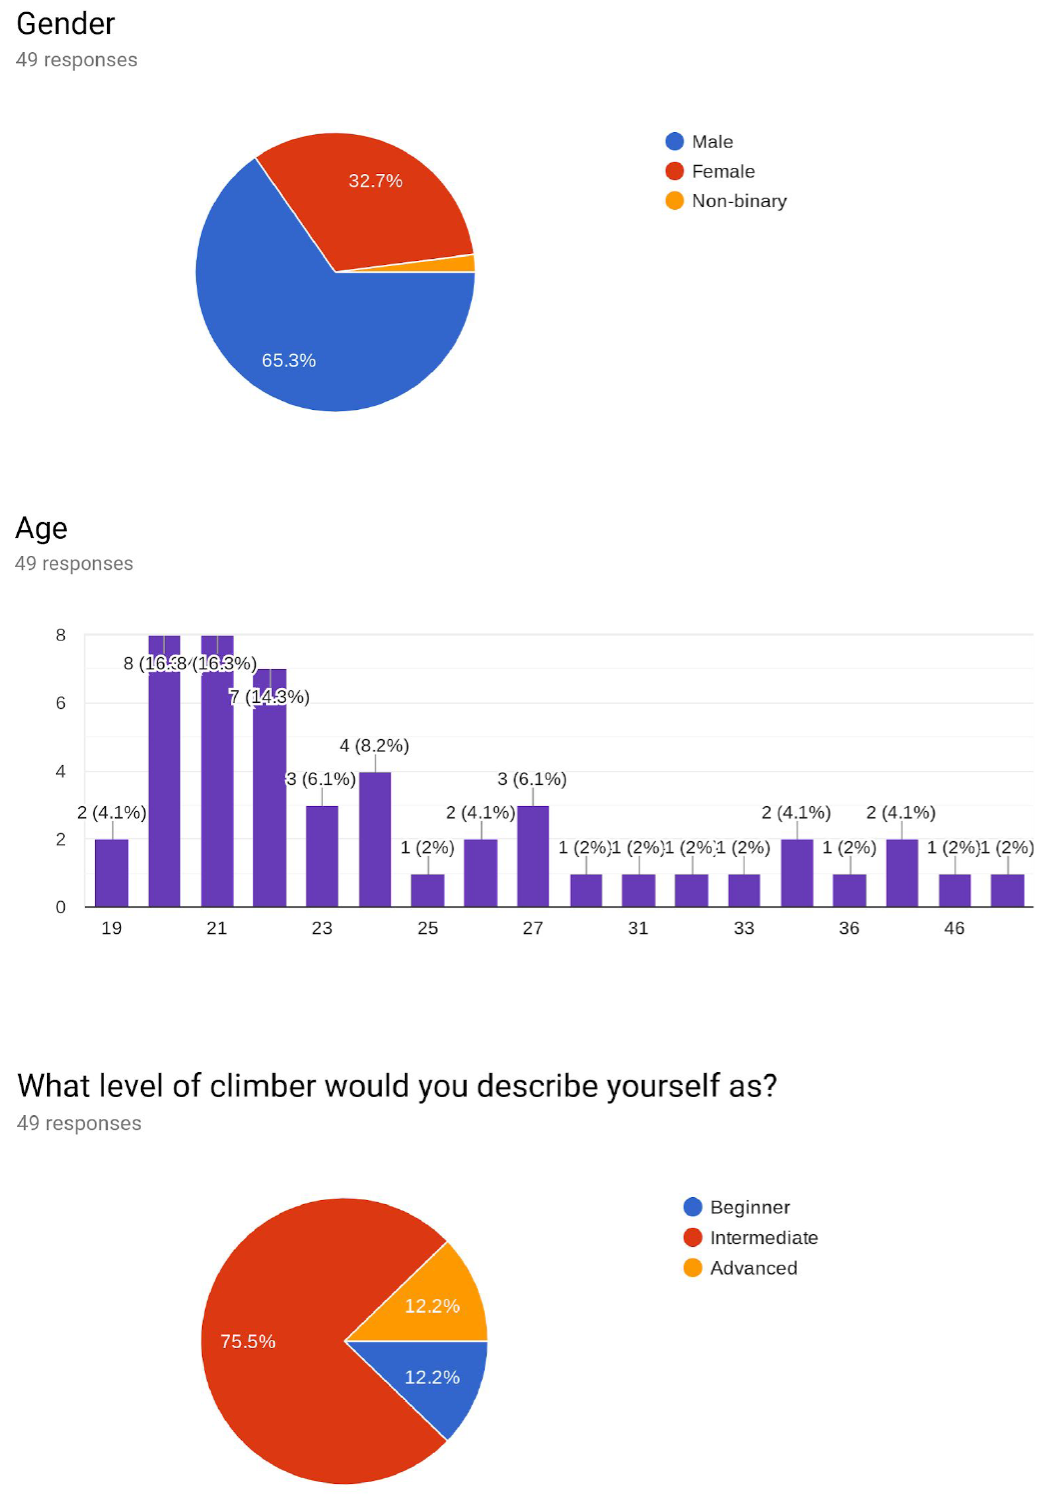
\includegraphics[width=10cm]{imgs/surveydemographics}
\caption{Demographics of Respondents to the Initial Survey}
\label{fig:surveydemographics}
\end{figure}
Some statistics on the demographics of the respondents can be seen in Figure~\ref{fig:surveydemographics}.

The male-female gender split is fairly consistent with the general indoor climbing population: 65\% male respondents compared to the 64\% stated in Rapelje's study on the demographics of climbers~\cite{climbing-sub-worlds}, and 65\% aged 19-24, compared to 60\% in that study.
This was aided by efforts to spread the survey link across a range of local climbing pages and Facebook Groups, not just the student groups to get a more representative sample of views.

With three-quarters of the respondents self-describing as intermediate climbers, the survey predominately hit the target audience for the project. 
Although all the responses were taken into account, a more heavy weighting was placed on the suggestions given by intermediates compared to the lower and higher abilities.


\subsection{Insights Gained From the Survey}
\subsubsection{Equipment Used}
To inform my decisions on what form my interactive device should take, I asked what items of equipment climbers often bring to the wall.
Everyone stated that they bring their own shoes, 90\% stated they bring a chalk-bag (a small hip-bag that contains powdered chalk for drying fingers and improving grip), and 31\% said they bring a small brush for cleaning dirty holds.

This provides a range of locations for locating a potential device, either inside the pocket of the chalk-bags, or attached to a brush, keeping with the light-weight aims of the project.

Only one respondent in this question included a phone in their list of equipment brought to the wall, and one even explicitly stated that they deliberately left their phone in their bag in order to "get away" from it. 
However, in later questions, an app (and thus a phone) was the most discussed potential device for usage, with multiple suggestions that a "you would severely limit your possible audience by having the need for a device" as "everyone has a phone" so I should "stick with an app".



\subsubsection{Communication With Others Whilst Climbing}
Because a potential use of the device was to aid some of the common interactions that climbers had with friends at the wall, two of the questions in this initial survey asked what kind of things people wanted to hear whilst climbing, and what they often told their friends.

The most common response was ``beta", which is a colloquial climbing term for advice on how body-positioning should be used to solve a tricky climb. 
This can vary a lot between climbers, with each climb usually having two or more potential solutions.
Also, being able to ``read" a climb to determine this beta is a tough and much-sought-after skill within the climbing community, to the extent that it is often nearly impossible for the very best in the sport, and thus definitely out of reach of any Artificial Intelligence (AI) I could hope to create within this project.
An alternative, which was suggested by a few survey respondents, could have been to record (with either video or other sensors) a proficient climber climbing that route, and then showing that at a later date. 
However, this data-collection and -replay contradicted my initial aim of the device/app being able to be used anywhere by anyone: for a low-cost app to be usable everywhere, the requirement to go to every climbing centre every few months and re-record somebody climbing every climb at each climbing wall, just for the product to remain usable, was not feasible.

Another common interaction highlighted by the survey was ``pointing out holds" to a climber, who is often so engrossed in the climb that they do not notice a certain location that they could put their hands or feet.
This has an obvious potential use-case for a device, by using a colour video and existing computer-vision algorithms for coloured-blob-detection to find and then audio-relay the location of nearby holds to a climber, so this was selected to be examined further.



\subsubsection{Requested Potential Features}
Arguably the most useful question was the one asking
\textit{``Are there any features you'd like to see in a training app or device?"}.
This elicited a very wide range of suggestions, from yoga and meal plans to VR-viewing of someone climbing alongside.
Many of these were either too simple (and could be achieved either by existing apps, or an online search), or far too ambitious in scope.

The most common request was a way to log climbs in some way, and although a few logging apps already exist, this feature was definitely required in some way alongside whichever novel features were to be developed.
Tracking progression and seeing gradual improvements over time is a typical characteristic of training in any sport, but instead of just listing climbs that had been done, a few respondents suggested that other metrics could be tracked, such as height climbed, frequent muscle groups used, and weak-points in technique that caused a climber to fall off at a certain point.


Many respondents emphasised that ease-of use was very important, so they didn't waste time climbing by clicking through the app. ``Large buttons for chalky fingers" were requested, alongside ``a minimum of two clicks between opening the app and using it".

The video-analysis of technique was mentioned by seven respondents, with a mixture of technique-tutoring, centre-of-gravity detection and limb-annotation suggested.
Both centre-of-gravity and limb-annotation could be feasible achieved with computer-vision, so those were taken forward to the WOZ testing phase.
However, if beta-detection has been ruled out as too difficult for CV/AI, then giving accurate technique advice is even further out of the range of potential features: with the high complexity of movements in the sport, years of learning required to achieve coaching qualifications, and the high risk of injury if incorrect, giving explicit advice about how to climb is not something that I wanted to go into with this project.

One metric that was proposed is the analysis of efficiency or ``smoothness" in a climb.
A commonly accepted signifier of ``good technique" is when a climber moves neatly and directly between each successive climb, without any jerky motions or unnecessary readjustments~\cite{centreofmass}.
An accelerometer recording could be used to determine this metric and thus this suggestion was also brought forward to the next stage of testing.


\subsection{Feasibility and Potential Limitation of Video Analysis}
The initial survey showed interest in using CV to either give feedback about climbing technique, or to point out where nearby handholds were.
To those ends, I began experimenting with using OpenCV to detect blobs in previous recordings of my own climbing.

Although some small success was had in detecting the centre of body mass, and some nearby coloured handholds, the wide variety of different lighting conditions and noise from the low-res camera made the detections very inaccurate.
Another issue that arose was that the code would analyse the video very slowly, even on my PC with a graphics card, so converting that to battery-efficient code that could run in real-time on a mobile device would have been extremely difficult.
Due to the time-scope of this project, and the aims being to iteratively develop something and analyse how climbers interacted with such a product, I was wary of spending too much time trying to get video-detection working.


\subsection{Wizard-Of-Oz Tests}
To determine the requirement for this video feature vs using an accelerometer to provide data input, a series of informal discussions and WOZ tests were performed at a climbing wall with 3 boulderers.
This involved me writing a script, and showing images of potential screen displays when they performed an action or climbed.

Now knowing the probable abilities of the CV's video-analysis, which was either to label limbs and centre of mass on a video output, or to state nearby handholds during the climb, I acted out both of those features in a WOZ format, and the results of that test was that they were determined to be potentially useful.
However, the labelled video feature was stated to be only slightly better than just watching a video playback, and the inefficiency of setting up a phone to point at a wall to call out handholds with some delay was not something that excited the climbers.

The WOZ prototype that involved having an accelerometer data showing up on a graph with some form of "smoothness rating" was received well in the testing, and I felt that it would be a good idea to explore that route with the iterative testing and design, whilst also working on some of the video analysis in the background.


\section{Iteration \#2: Acceleration}
This section will outline my second large iteration.
Now hat I had completed the first iteration, with WOZ prototypes, and roughly knew which features and form-factors the users wanted, I next had to design and implement a real-code prototype to test.
In order to do this, I had to make some choices regarding the tools I'd be using, then make a minimal app that could record some data, before exploring different output options with my testers.


\subsection{Fundamental Early Decisions for Development}


\subsubsection{Platform Choice}
Despite researching a variety of different devices and form factors, one of the key aims of the project was always to make the final product as accessible as possible, therefore a OS-independent mobile app was decided upon after reviewing the survey results.
By not using any extra equipment such as wristbands or 3d-cameras, the scope and ability of the final product could be limited (by lack of sensors and processing power).
However, limiting the need for anything but just a phone, which almost everyone owns, was a worthwhile sacrifice.
As well as making user-testing much easier, this choice also helped narrow down the direction of the project: working solely within the limits of what a mobile app could achieve meant that the capabilities of that platform could be fully stretched and explored.

The two inputs that mobiles can easily capture, and that would potentially be most useful for the analysis of climbing technique, were video recordings and accelerometer data.
Video recordings can be analysed with various Computer Vision (CV) techniques and accelerometer data can be shown on a graph and analysed statistically to provide various outputs.

\subsubsection{Tool Selection}
\paragraph{App-development tool}
Next was to find a app-development tool that is quick and easy to use (for quick repeated iterations of the app), can easily import or link to the OpenCV Library (for the CV aspect), and is platform-independent (so any mobile phone owners can use the app, irrespective of OS).

Unity was chosen as it meets all three of those requirements, with a wide variety of ``Assets" (downloadable open-source libraries) that can be imported.
 
By providing a platform for creating simple user interfaces that could be exported to a range of platforms, and easy linking between the UI elements and back-end \verb|C#| code, I knew that quickly building and iterating over multiple app designs would be possible.
Also, having used Unity for games development in the past I was very familiar with it, so compared to potentially wasting time learning how to use other tools, this one met all the above requirements, with the added benefit of previous experience using the tool.

\paragraph{Version Control}
For version-control I used \verb|git|, backed-up on GitHub.
Being a one-person project I rarely bothered with the overhead of using different branches, but the ability to roll-back to working code and releases, and to \verb|stash| and \verb|pop| various files at different times was very useful during development.
Once or twice a week, after a new feature or big set of fixes had been added, I would up-version the app, and release a compiled .apk binary to the project's GitHub page.
This allowed the easy re-installing of older versions when trying to locate a bug, as well as a clear documentation of all fixes and features included at each minor version upgrade.




\subsection{First minimalistic app: Recorder}
After the success of the accelerometer idea in the previous iteration's tests, I decided to build an app based around this, to use in some real in-field testing.

This first app just had a two buttons, START and STOP, which would, respectively, start and stop recording the mobile phone's raw accelerometer data into a \verb|.csv| file.

\subsubsection{Axes Selection}
The accelerometer's API allowed me to collect data from each of the individual axes, so it seemed like a good idea to use this to determine and compare acceleration vertically vs horizontally, which was a potentially useful feature.
However, after viewing the raw data output from the first climbing session, it became clear that the phone's axes would very rarely match up with the real-world axes in any meaningful way, and even some sort of calibration at the start of the climb would quickly become meaningless as the climber rotates and moves up the wall.
% , as can be seen in in Figure <<>>.
% <diagram/pic of phone axes whilst in climbers pocket>

Therefore just the total magnitude of the vector-sum of the acceleration measured along all three axes was used going forward.

\subsubsection{Mock Output}
During this first test, the lack of an in-app output was an obvious limitation, but after a climbing test session with just this feature, I was able to copy the data into a spreadsheet software and graph the results, giving Figure~\ref{fig:twoclimbsgraph}.

\begin{figure}[h]
\centering
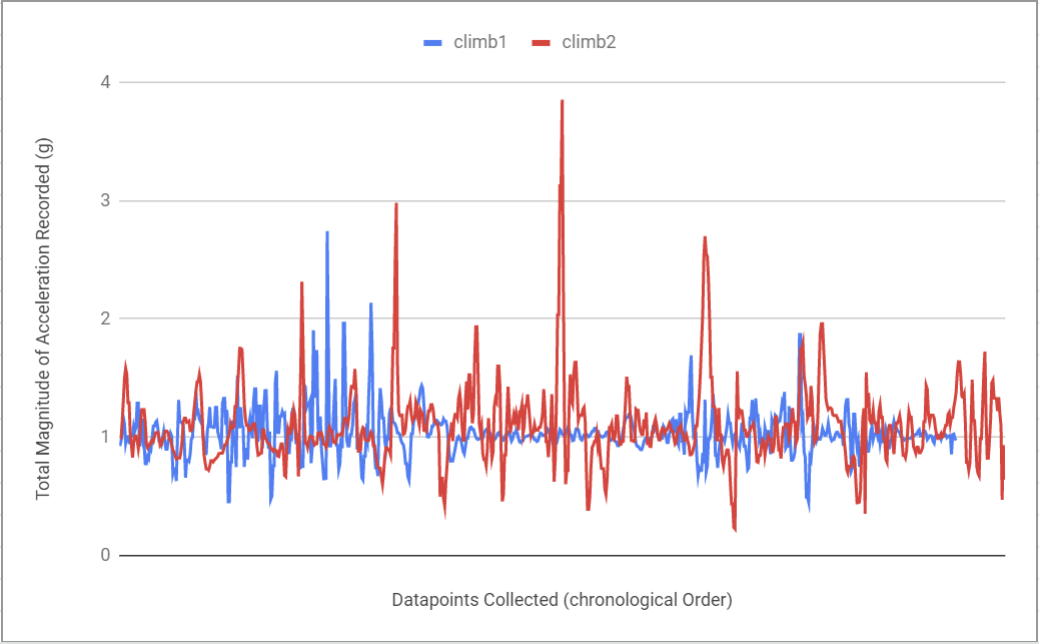
\includegraphics[width=12cm]{imgs/graph_two_climbs}
\caption{Overlaid Graphs of the Accelerometer Data Recorded During Two Different Climbs}
\label{fig:twoclimbsgraph}
\end{figure}

I then met up again with the climbers from that test-day at the wall, and we discussed the graphs and could recognise which climbers were climbing which climbs, just from the spikes on each line graph; this was the first time I saw a clear correlation between the acceleration and the climbing style and ability, an exciting result.

\subsection{In-App Statistics}
The testers enjoyed viewing the graphs I had produced, so I started working on adding graphs to the app.
Unfortunately here I hit the first limitation of the tool I was using - Unity.
Primarily designed as a Games Engine, Unity didn't have an easy method of plotting graphs, and any Asset Store solutions were expensive to buy. 
A solution involving drawing dots on the screen for every data point, and calculating the size and angles of lines connecting them was possible, but I knew that would take a few days of coding, and wanted to iron out any potential kinks in my data-collection methods before investing that much time into coding.
Also, I had another testing day scheduled with my climbers, so wanted to quickly code a simpler form of output to see how they interacted with the data.
Simply calculating the min and max acceleration, and the time taken to climb, only took a few lines of code, and so the second prototype of my app included a screen that would display those statistics after a climb.

During the test session, both of the people I was climbing with enjoyed using their max acceleration in a fun and competitive manner.

They took it in turns trying to produce as much acceleration, or "power", as possible on some climbing moves, and also compared times whilst slowly doing easier climbs, trying to keep their max acceleration down to as low a score as possible, and doing certain climbing moves with as much or as little speed as possible.
When the potential of a "smoothness" score was brought up in discussions, they told me that a statistic other than just max acceleration, and more closely linked to actual climbing technique, would be very useful.

\subsection{Development of Smoothness Score}
Seeing a range of graphs on the spreadsheet software (similar to Figure~\ref{fig:twoclimbsgraph} but with many more climbs) was very interesting.
Some climbs' graphs were consistently fluid with no big spikes, some were mostly flat with a few large spikes, and some had a lot of small spikes, which clearly showed that there were discernible differences between the accelerometer data produced by different climbs, something I intended to utilise.

After discussion with some climbing coaches, they suggested that what they often tell clients to do is to climb the same easy climb repeatedly, aiming for as fluid and smooth a motion as possible.


% Add new figure here for this discussion
% NOTE -  maybe re-do the climbing graphs to show three good examples? 
%This is clearly visibly in the 1st


Alongside this, occasionally some harder climbs call for bigger ``dynamic" moves, but accuracy in catching the holds without lots of small adjustments is still important for good technique.
% This style of climb can be seen in graph 2 of figure <?>.


What the coaches I spoke to said they would generally judge as a climb with poor technique is one where many small inefficient and jerky movements were made: the repeated re-gripping of holds can lead to early forearm tiring, and the uncontrolled and ungainly fluctuation of momentum of the overall body mass is very inefficient.
One aim of good climbing technique is to prevent this early tiring, and reduce as much inefficiency in movement as possible, as these are often the factors that prevents the successful summit of a harder climb.
%citation?

However, because climbing technique and style can be very variant among both climbers and between each climb on a wall, there was no way to provide an accurate "best" or "aim" score, especially when variations in the acclerometer recordings on different phones is taken into account.
Instead I opted to try and find some form of quantifiable metric that, as the testers had suggested, was more closely linked to climbing style than just minimum or maximum acceleration, yet didn't have an absolute limit or goal, to keep the flexibility required between different climbs and different sensors.

\subsubsection{Four Alternatives}
Although previous studies\cite{climbaxstudy, climbbsn} use machine-learning techniques to train classifiers that can predict ability, attempting to directly analyse the smoothness of a graphed acceleration data-set to distinguish between climbing styles has not previously been attempted.

I decided to test out a range of different options, on real climbing data, to determine which score was the closest representation of climbing style.
To aid with the comparison of climbs, the metric should be able to distinguish between different styles: if a climber is repeatedly trying to climb as statically and smoothly as possible, then the score should be able to reflect that by changing in a predictable manner.

\paragraph{Mean}
$$\frac{\sum n }{N}$$
The simplest statistical measure was worth testing: a large amount of higher accelerations would result in a higher mean, which would possibly show differences in climbing style.

\paragraph{Variance}
$$\frac{\sum (n - \bar{n} )^2 }{N-1}$$
Again, a classical statistical metric that had potential: measuring how varied the accelerometer data-points are is linked to the above discussion on how more ``spiky" graphs often portray less smooth climbs.

\paragraph{Average squared difference between each consecutive data-point}
$$\frac{\sum (n_i - n_{i+1} )^2 }{N}$$
Taking variance a step further, and calculating the pairwise differences in the dataset could give a good measure of how ``jumpy" the chart is.
By measuring the differences in acceleration, this statistic works in much the same way as finding the average squared ``jerk", which is the derivative of the acceleration.

\paragraph{Single-Lagged Auto-Correlation}
$$
\frac{\sum(n_{i} - \bar{n})(n_{i+k} - \bar{n})}
      {\sum(n_{i} - \bar{n})^{2} }
$$
My idea for using this metric was that if each data-point is closely correlated with its successive data-point, then the overall line would have less jolts, but run in a more smoothly varying way.

\subsubsection {Comparative Testing}
I had three test climbers climb three different routes, in either a deliberately static style, a deliberately dynamic style, or their usual style: a hybrid of the two.
Using the data recorded from these climbs, I calculated each of the above metrics, visible in Table~\ref{tab:smoothnesses}.

\begin{table}[h]
\centering
\begin{tabular}{|c|c|c|c|c|c|c|c|c|}
\hline
climb  &  climber & style & min & max & mean & var & var-diff & lagged-autocorr \\ \hline
purple v0 route & 1 & static  & 0.29 & 3.50 & 1.10 & 0.12 & 0.06 & 1617.90 \\ \hline
purple v0 route & 3 & static  & 0.07 & 6.39 & 1.09 & 0.16 & 0.12 & 1600.46 \\ \hline
purple v0 route & 2 & dynamic & 0.16 & 10.96 & 1.11 & 0.39 & 0.18 & 2150.63 \\ \hline
purple v0 route & 3 & dynamic & 0.20 & 9.76 & 1.14 & 0.40 & 0.16 & 1931.72 \\ \hline
yellow v1 route & 1 & static  & 0.21 & 2.20 & 1.06 & 0.05 & 0.02 & 795.96 \\ \hline
yellow v1 route & 1 & hybrid & 0.06 & 11.41 & 1.06 & 0.17 & 0.11 & 2176.12 \\ \hline
yellow v1 route & 1 & dynamic & 0.03 & 8.20 & 1.07 & 0.21 & 0.10 & 1862.94 \\ \hline
pink v2 route & 2 & static & 0.45 & 2.74 & 1.04 & 0.04 & 0.03 & 793.59 \\ \hline
pink v2 route & 2 & hybrid & 0.21 & 4.04 & 1.05 & 0.08 & 0.03 & 1939.77 \\ \hline
pink v2 route & 2 & dynamic & 0.16 & 10.32 & 1.12 & 0.25 & 0.15 & 1826.36 \\ \hline

\end{tabular}
\caption{Comparison of Smoothness Score Candidates}
\label{tab:smoothnesses}
\end{table}

As can be seen, despite both the var-diff and the lagged-autocorr algorithms showing some promise, the only metric that can reliably distinguish between the three styles of climbing is the variance, so this is the score I took forward.

\subsubsection{Confirmatory Testing of Variance}
In the app, I added a calculation at the end of the accelerometer-recording, which would display the variance to the user on the app screen immediately upon completing a climb.

Taking this back to the test-users, they agreed that this metric was much better for them being able to compete on a climb, both with themselves and with each other, to get "as static a climb as possible", meeting the requirements for this score.

One point they did raise was that comparing a score of, for example, $0.21234$ and $0.17018$, felt odd.
My testers found comparing and discussing numbers in the 20-100 range much easier and more natural, so on the next iteration of the app, before displaying the variance I multiplied it by a hundred and displayed it as an integer.

\subsection{Graphing Acceleration Data}
Now that I had a working "score" that I could analyse user interaction with, I moved onto the next feature that my testers requested: plotting and showing a graph of the accelerometer data in the app.

\subsubsection{Timing Issues}
For the first version of my graphs, I simply plotted a rudimentary scatter-graph:
within a given box on the screen, for each data-point $n$ in the accelerometer recording, I drew a small circle object $n$ pixels up, and spread the dots across so they stretched to fill the width of the box.

Although this resulted in what looked like a line-chart with time as the x-axis, there were a few issues that arose when I took this version of the app to be tested;
the graphs that were being displayed didn't quite ``look right".
Although the x-axis of the graph was supposed to represent time, because I wasn't recording the actual time but just successive data-points, the x-axis didn't truly represent time in the real-life stress-testing that climbing involved.

What I found out to be happening was that the way Unity handles incoming accelerometer data was to record it as fast as possible - which is exactly what a developer would want if they were using it as an input to a game.
However, this caused the side-effect of the time-scale varying slightly, in a usually unnoticeable manner.
During at-home debugging, when I recorded a timestamp to the csv file alongside the accelerometer data, the time differences only varied from 0.004s to 0.006s, and although this would obviously need to be fixed for the accuracy of the graphs, it didn't explain how the graphs when climbing would be so inaccurate.

Taking this code back to the the climbing wall a few days later, I discovered that during some more dynamic climbing moves, the differences in recordings reached up to 0.5s.
Upon closer inspection, I saw that when the phone was detecting a very large acceleration along with a large rotation, it would try to change the display orientation, resulting in a brief pause in the recording of the accelerometer.

Therefore, to fix these issues, I forced the app to remain in portrait mode, and re-wrote the recording function caller to ensure that exactly 20 samples per second would always be recorded.

Despite fixing this consistency of timings, I also re-wrote the graph-drawing code to take into account the associated timestamp for each point.

% \subsection{Using Lines instead of dots}

% (is this section necessary?)

% The dots graph had some gaps in, so testers asked why not use lines.

% (could describe the pair-wise datapoint trigonometry with a few diagrams, and screenshots to show improvements)


\subsection{Viewing Previous Climbs}
Up until this point, the statistics and graphs of each climb had been only visible directly after a climb had been completed, and to compare climbs the users had to memorise the previous climb's smoothness score and roughly how the graph looked, to then hope to improve.

Viewing a list of all the previous climbs, with associated smoothness scores and graphs, was the obvious (and much-requested) next feature to add.

Because of the way that I had been saving the accelerometer recordings to the phone's persistent memory for debug purposes, I could scrape that folder for all csv files, and populate a scrolling list with a set of graphs and smoothness scores.
See Figure~\ref{fig:scrollview} for the final display of this.

\begin{figure}[h]
\centering
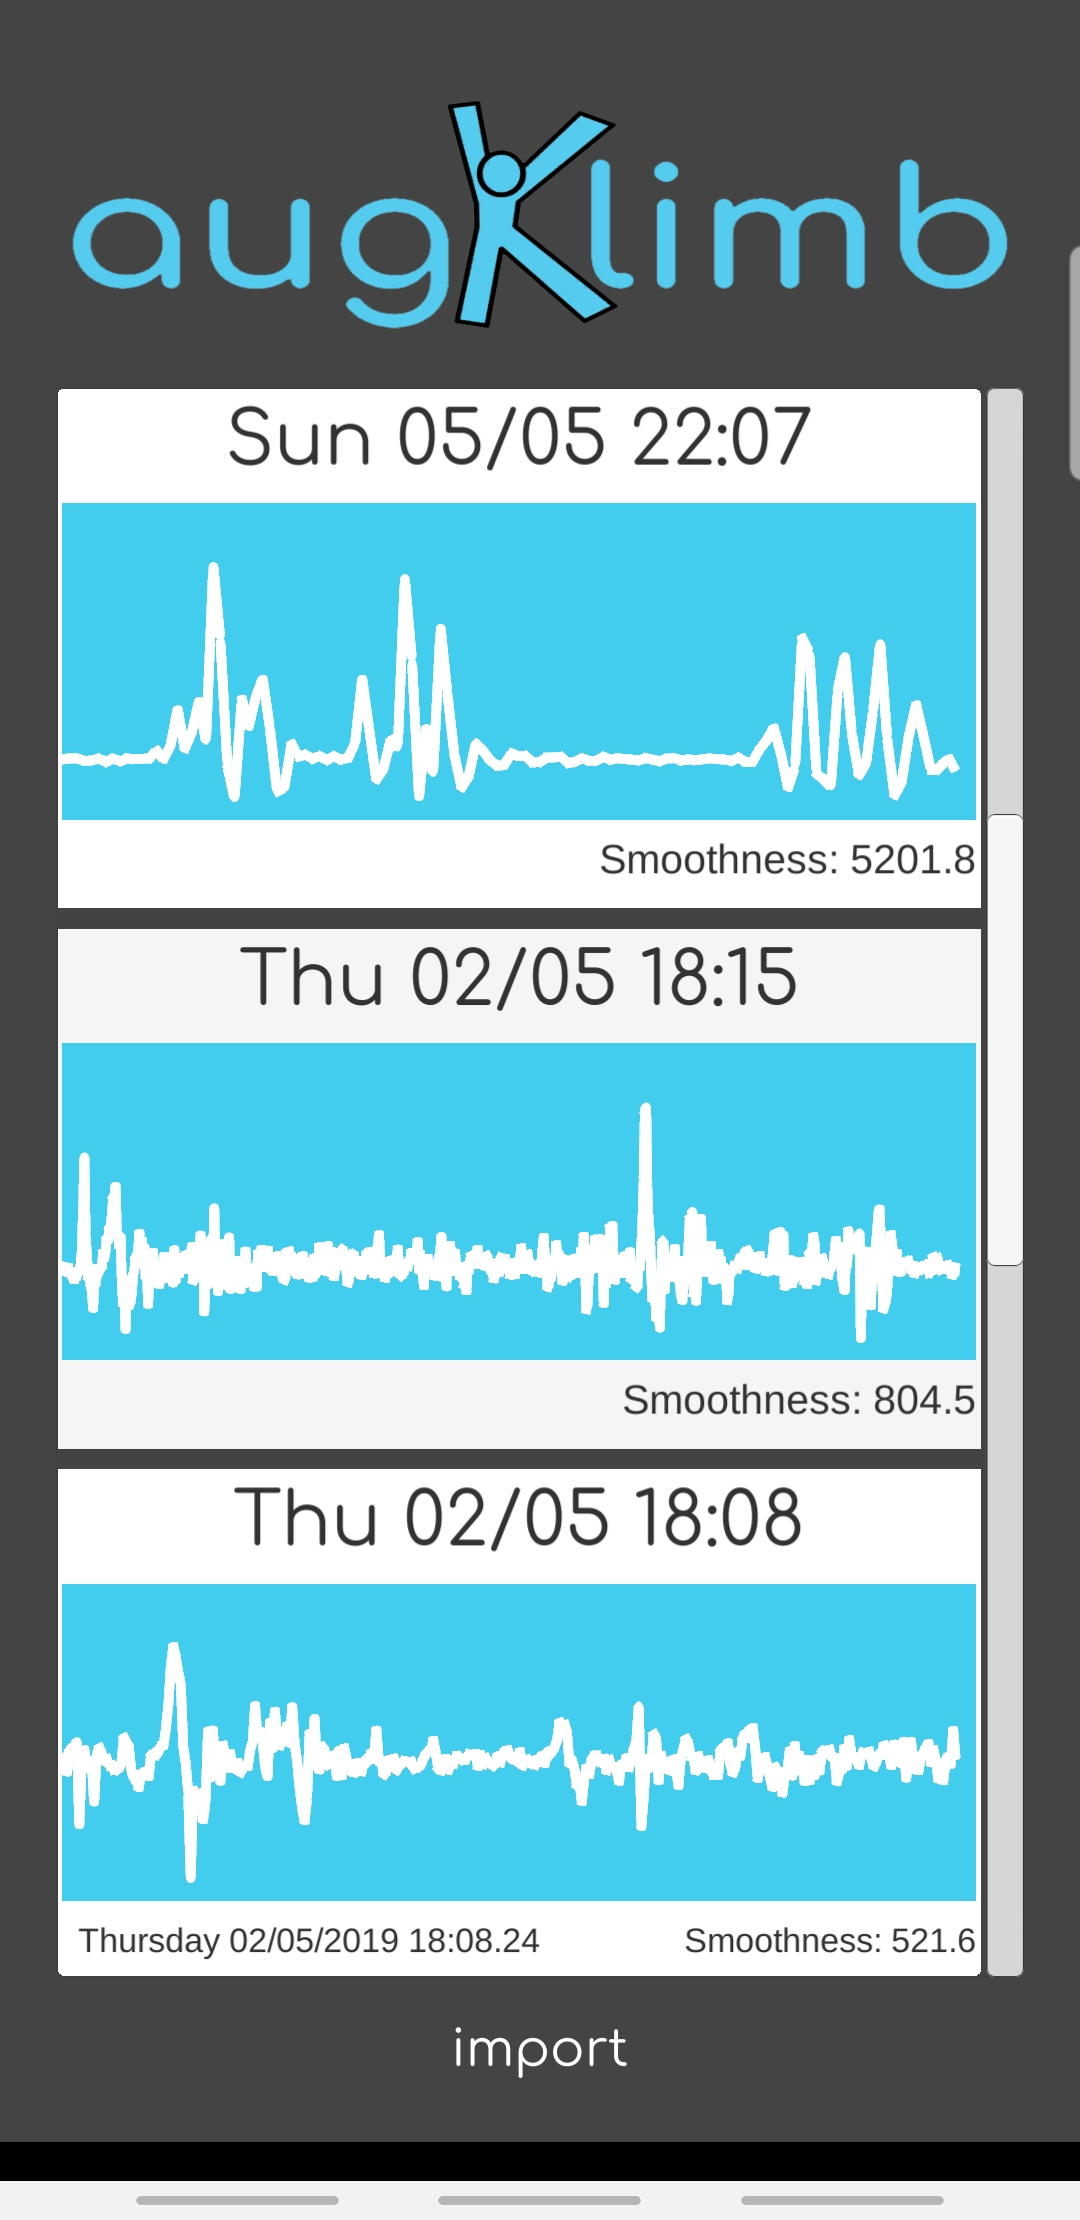
\includegraphics[width=6cm]{imgs/scrollview}
\caption{augKlimb's scrolling view-all-climbs page}
\label{fig:scrollview}
\end{figure}


\subsection{Viewing Individual Climbs}
By viewing how my testers used this scrolling view, to compare previous climbs' graphs and smoothness scores, I also noticed that they would occasionally touch a climb's graph with a finger.
When asked about this action, they told me that they had instinctively clicked, with the expectation that they could load that specific climb and view more information on it.
Therefore I added another page into the project (see Figure~\ref{fig:singleclimb}), to view an individual climb's graph in full-screen detail, with more statistics like smoothness and time taken all on that screen.


\subsubsection{Horizontal Scale}
With the full-screen view of an individual climbing graph now possible, a discussion of scale was needed. 
Whereas in the scroll-view of all the climbs, the graphs were scaled to fit the whole data-set inside the given box (again see Figure~\ref{fig:scrollview}), one of the main expectations of the per-climb graph view was that graphs would be "zoomed-in" to see more detail.
After some testing it was found that a scale of 100px per second was optimum for viewing the acceleration's spikes with enough clarity whilst also not making the longer climbs to have an excessively long scroll to view. 

\begin{figure}[h]
\centering
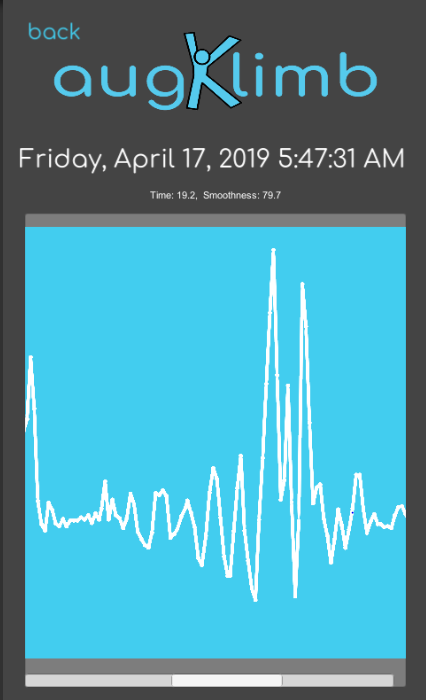
\includegraphics[width=6cm]{imgs/singleclimb}
\caption{augKlimb's single-climb-viewing page}
\label{fig:singleclimb}
\end{figure}




\section{Iteration \#3: Video}
In this section I outline the third major iteration cycle: the incorporation of video footage and frame-by-frame playback linked to the acceleration graphs created previously.


One tester had suggested that as it was now possible to scroll horizontally through a climb's graph, using that scrollbar to also view frames of a connected video file could be a useful feature.

One option would be to use the phone to record a video, and get the accelerometer data from a wristband or other device.
However, keeping in with the theme of accessibility and only using a mobile app, the idea of connecting two mobile phone devices, so a friend with the app could video-record you as you climbed with the accelerometer feature, was chosen.


\subsection{Networking Options}
A variety of different options for networking two phones together was explored, including Unity's built-in Networking, Wifi-Direct, uploading to the Cloud, and Bluetooth.


These options had varying levels of support through Assets on Unity's Asset store, but after looking through reviews most of them were deprecated, broken, or did not fit my needs.
Those that potentially did cost upwards of \pounds50, which is not something I was willing to pay for a library of code that may not do what I needed.

Thus, I would have to code my own solution.


\subsubsection{Unity's Built-in Networking}
The only one of the above options that is provided in some way by Unity is the Networking libraries.
At first its probable ease of use seemed like a good option, and despite having some issues using it in the past (during my third-year Games Project)I knew how to connect various devices together.
However, the UNet library provided by Unity had just recently been deprecated, and the replacement networking service was under development at the time of writing this, so documentation was often unavailable or incorrect.

Also, despite the ability to link two phones whilst I was at home, when at the climbing walls this presented an issue as the free WIFI provided at these wall often blocked LAN connections between devices.

\subsubsection{Cloud}
Uploading to cloud would require coding some sort of scalable server and storage, something I could definitely do, but this level of overhead for what should just be the sharing of files and syncing between two devices that are located physically very close together felt like an unnecessary amount of work and time spent.
Also, it would have been very slow to upload and download a video over the web for every climb, whereas a solution that could utilise the close physical locations of the devices to transfer files faster.

The requirement to add some sort of user profiles, or unique code to differentiate and request the correct download, was a big added complexity, yet one that could have given an added bonus of users' data being backed up to the web and usable in other ways, for example from a web platform.
Although this may be something to look into in the future a cloud server isn't the solution to this specific problem, and is not really within the scope of this project.

\subsubsection{Wifi-Direct}
Wifi-Direct enables the direct connection and file-transfer between compatible devices
Although this seems like a great technology, and could be ideal for this specific use case, the few docs I could find online that detailed using Wifi-Direct with Unity stated that many parts of this feature had been deprecated, and was closely linked to the now-obsolete Unity Networking API.


\subsubsection{Bluetooth \& NFC}
An idealised use-case for the app that presented itself in WOZ testing was to just bump two mobile devices together, ``pairing" them using NFC, and then using the longer-range Bluetooth to transfer a sync command and any video or data files.

Unfortunately, this uncovered a large issue with using Unity as my tool of choice - no support or libraries for either Bluetooth or NFC. 
Even the single free Asset online was broken, leaving me with one solution: to write my own \verb|Java| plugin using Android Studio to connect the NFC and handle Bluetooth file transfers, then expose public functions in a compiled \verb|.jar| file that the \verb|C#| Unity code could then connect to.

After spending a few days writing this code, it worked occasionally, but the interplay between the two sets of libraries, on a variety of Android devices, was just too unstable.

\subsubsection{Native Messaging}
Both Android and IOS provide easy APIs for sharing files via social media or email, which is utilised by the free NativeShare Asset I downloaded from the Unity Asset Store.
Using this library, the JSON representation of each climb could easily be shared between devices using a messaging app, which was enough of a solution to this problem to allow me to take it to the testers and determine whether a more streamlined solution was needed.

During testing, climbers could record a climb, view it, and then hit the Share button to send that file to a friend, who could import that file and view it on their phone.
Despite the time spent on unsuccessfully trying to get Bluetooth working with my plugin, by simply using this same button, my testers could use Bluetooth instead of the messaging app to send the climb files - a slightly more convoluted approach to simply bumping two phones together, but one that worked more reliably when Bluetooth stopped working, which it did occasionally on one of my test devices.


\subsection{Video Player}
Now that there was a way of sharing climb-data-files, it was time to add the video-scrolling feature.

By changing the climbing graph view to shrink down to half the page, and adding one of unity's VideoPlayer components in the top half of the screen, the video could play.
Then, to set the frame of the video to display, the graph's scrollbar's position could be queried, and translated into a frame-number, which was set on the player.

Everything seemed to work great, and the testers really enjoyed it:
I would record them climbing with their phone in their pocket, then send them the video via messenger, they would download and attach it, and then could view and scroll through the video frame-by-frame to see which spikes in the graphs corresponded to which moves.

\subsubsection{Timing Issues}
However, the two recordings (video and accelerometer) would have to be started at precisely the same time in order for the timings to match up.
There was, at first, some potential in scraping the video-file's metadata for a timestamp, and matching that timestamp with the times in the recording; unfortunately when the videos are sent via the various messaging apps we were using, they would be transcode the video - to save data whilst sending, I assume - which would strip all useful metadata and timestamps.

Therefore, instead of automatically time-matching a list of recorded videos with a list of climbs, a video file would have to be manually selected and added to a climb to associate the two - an unwanted but necessary extra step for reliability.
Also, a manual ``Video Offset" selector was added above the video-player, so users could adjust the time-differential between the graph and video so that they could scroll in time if the automatic metadata-scraping and timing-detection failed to predict the correct time difference upon manual matching.
To aid this automated system, any video recordings made via the app would save the exact timestamp (to millisecond-precision) into the video's filename, which is not always changed when these messaging services transcode the video.

\subsubsection{Video Player Bugs}
Through this testing of a variety of video-sending methods, I discovered a bug:
on some devices, some videos, in some orientations, with some video-formats, would cause the video player to fail.
This is one of the toughest bugs I have ever had to fix, as it was very nearly un-reproducible: If I changed any one of the four requirements above, the bug would disappear, and if I changed the scaling settings in the \verb|VideoPlayer| component then a different combination of the settings would cause it to fail instead.

Most often, the use-case that produced this bug was when a video recorded on a phone was matched with an externally-imported climb-file.
Unfortunately, that was a very common use-case for my testers.
Whether the video was recorded through the in-app video recorder, or the phone's native camera app, it would usually fail.
If that video was sent via a messaging app, then re-downloaded off that app, it would work.
If that video was rotated and then rotated back again, it would work.

This was frustrating, as surely if a video was recorded on a device, and playable by that device, Unity should have access to the codecs required to correctly play that video?
In total, around two week's worth of development time was spent just trying to figure out how to play video reliably, as it would be very frustrating for the testers when they'd get down off a climb expecting to analyse the graphs and visualise the climb frame-by-frame, only for a flashing screen to greet them.

Eventually I completely changed how the videos were being played in Unity to solve this issue: instead of using a simple VideoPlayer component, I attached a second camera to the VideoPlayer API, and then scaled and rendered that camera's view onto a mesh in the view.
This more convoluted way of displaying video wasn't as smooth to playback the video, and delayed when searching for a specific frame, especially on older devices, but the decision was that a flickering video feed was better than an unreliable one.



% Turning off multithreaded rendering makes video playback much smoother, but results in the frame not jumping to the selected one as easily, or at all, on slower android devices.

\subsection{Testing}
The testing phase of this major iteration was successful: users enjoyed viewing the video footage alongside the graphs, and made a few other suggestions for UI improvements for the next stage too, but the app was nearly ready for deployment.




\section{Iteration \#4: Final Improvements and Deployment}
Now that the app was relatively stable and the two big features (acceleration and video) were working well together, it was time to clean the code with a refactor, implement the list of small requests that my testers had been suggesting, and then deploy the app, publishing it on the Play Store.

\subsection{Code Refactor}
Because I was starting to send climbing files between devices, I needed a more reliable way of exporting and parsing those files, especially with the added complexity of having video-paths and other information attached to them, the plain \verb|csv| files were not sufficient.
Also, having gradually built up the app with a script file per-view, for example one script to handle the recording and another to handle the viewing, as I added more features and file information, the code-base was getting convoluted.


\subsubsection{Refactor}
Therefore, I completely refactored all the code, keeping the only the minimum logic required for each view in those files, and splitting out all file-handling and graph-drawing methods into separate classes, along with creating a new \verb|ClimbInfo| dataclass to store the accelerometer data, title and associated video information.

Now that all the data associated with a climb was contained in a single class, I could utilise Unity's built-in \verb|Serialization|, which could automatically convert a correctly setup class directly into a \verb|json| file, and visa-versa. 
This was complex to achieve, but it proved very useful later on when adding more information to my ClimbData class: I no longer had to maintain my own file-saving and file-parsing code, but could rely on the serialisation to work with the files.


\subsubsection{Caching}
This refactor also gave me the chance to fix some performance issues that some of my testers had been having after using the app for multiple sessions.
As the number of climbs increased, so did the time it took to populate the list of climbs, as each file had to be loaded, and each graph drawn, before that page of the app could load.
Caching a list of \verb|ClimbData| objects prevented this repeated file-loading, but caused some issues with cache invalidation:
\begin{itemize}
    \item When loading the app for the first time, all of the climb-files in persistent storage should be read and cached.
    \item When a new climb is recorded, it should be saved to persistent storage and also cached.
    \item When an external climb-file is imported, it is first loaded into memory, then should be saved both to persistent storage.
    \item When a climb file is edited, it should be overwritten in persistent storage, but is already cached so should not be re-added to prevent duplicates.
\end{itemize}
This all took a lot of working out to cover all edge-cases, but the eventual solution involved tightly coupling cache-updating with the action of saving to disk, and decoupling it from any loading functions, checking for duplicates before adding to the cache, and adding an auto-initialisation feature to the cache:
If the cache is empty when queried, it will contact the \verb|FileHandler| and populate itself with a list of \verb|ClimbData| objects corresponding to what is in persistent storage.


% Infinite loop caused by self-initialising cache being updated by loader, which then causes the self-initialisation again. - selfinitialisaion checking for null, then reeiving full list, rather than asking for its list to be populated. Tied cache-updating to the saving of files instead of the loading of files.


\subsection{Testing-driven UI Improvements}
Alongside the video feature being developed and tested, my twice- or thrice-weekly testing sessions had provoke a range of smaller UI tweak and improvement suggestions, so I implemented all of those as I prepared the app for the first full deployment:

\subsubsection{Countdown}
One of the earliest of these was that starting recording as soon as the START button was pressed would record the acceleration caused by the climber putting their phone in their pocket and walking up to the wall.
To prevent this, a five-second countdown timer was introduced before recording commences, accompanied by a vibration so that the climber could have time to set up and know when to begin climbing.

\subsubsection{Guides}
Also, a lot of questions were asked when climbers first started using the app, so alongside a guide and FAQ on the website, I added clearer button names and brief descriptions at the bottom of each page to describe what happens with each feature.


\subsubsection{Cropping}
Sometimes when reaching the top of a climb, testers would just jump off, and land on the floor.
This created a large spike on the accelerations graph, and had a resultantly large impact on the smoothness score.
Thus a button was added to "crop" a climb's graph.
The horizontal location of the scrollbar was detected, and after a confirmation from the user, any climbing recording data after that point would be removed.

\subsubsection{Deleting}
To keep down clutter, testers had previously requested the ability to delete old or mis-recorded climbs, so now that each climb had its own page, a button was added that would remove the currently-open climb from the device.


\subsubsection{Back Button}
For Android, I removed the in-app back button, instead using the native OS's API to detect when the phone's back button had been pressed and returning the user to the previous screen, integrating the users' usage more closely to what they are used to from other apps.



\subsection{Publishing to Google Play}
As I don't have either a Mac or an iPhone, despite my choices to use a platform-independent software tool, I was only able to build to Android throughout this project.
That meant that the natural distribution service to use was Google Play.

Publishing to that store required a developer account, images of the app in use, various review procedures, and for me to write both a code of conduct and a privacy policy.

This Play Store listing can be seen \href{https://play.google.com/store/apps/details?id=com.lukestorry.augKlimb}{here}, with a screenshot in Figure~\ref{fig:playstore}.


\begin{figure}[h]
\centering
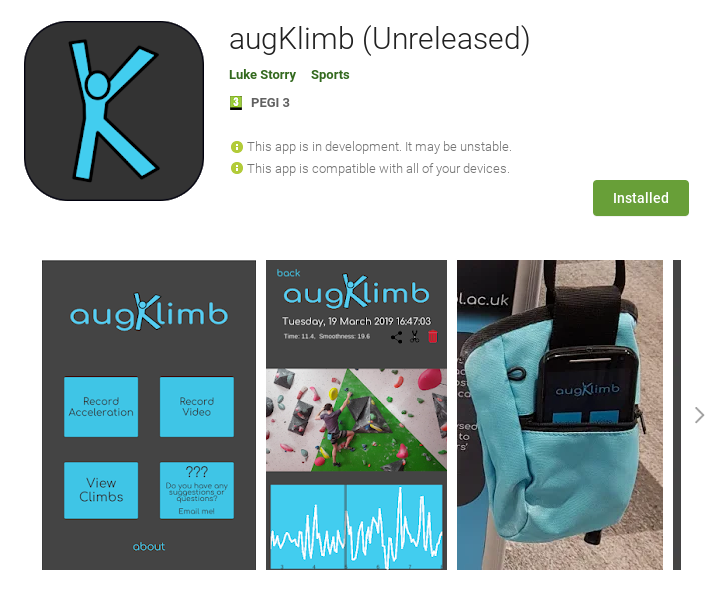
\includegraphics[width=9cm]{imgs/playstorescreenshot}
\caption{Screenshot of Play Store Listing}
\label{fig:playstore}
\end{figure}

To ensure that the general public did not have access to the test versions of this app, but only participants who had consented to be a part of this study, I did not release a full production version of the app, but used Google's Limited Beta Rollout feature to only provide beta access to the testers that I had given links to.


\subsection{Easier testing}
One obstacle that all my testers had faced throughout the project was how to install the app.
With such an iterative development processes, I was recording the app every day and trying two or three different versions each week.
This required either me lending one of my mobile devices to the testers to use, or side-loading an \verb|.apk| file onto the users' phones, disabling various security measures to install the app each time.

Having the app on Google Play not only made it a lot easier to upgrade the app on everyone's phones before each testing session, but the added legitimacy provided by not having to side-load the apk meant that a wider variety of people felt comfortable installing the app from a provided link.
This caused the amount of testers who were regularly using and testing the app to increase from 4 to 15, providing a rich variety of feedback from regular users of all abilities, both through occasional conversations and through the feedback form I had linked to the homepage of the app.




\subsection{Smaller Test-led Refinements}
Having more testers, each using the app slightly differently, led to a wide range of feedback, advice, and suggested improvements.
Also, the testing being on an assortment of different devices highlighted a range of small bugs that were either non-existent or at least infrequent on my own devices.
Few of these are worth mentioning, usually just requiring corrections to button-placement or changing the configuration of the file browser.
One bug caused a permissions error on Nexus devices, but after a week of helping that user manually re-enable the correct permissions, Unity released an update that fixed what turned out to be a bug in their engine.

\subsubsection{Title Editing}
Until this point, the title of a climb had just been the date and time that it was recorded.
In the initial survey, a climb-logging app was requested, and so to meet that demand I added the ability to edit this title to name the climb's grade, colour, and location.

Some testers didn't use this feature as they weren't interested in creating a list of climbs, just analysing the specific one they were working on at the time, but for others this added a nice way to be able to scroll back through climbs from a previous session and easily find one to replicate or compare to.


\subsubsection{Video Recorder}
Despite previously having moved away from recording videos within the app, and instead just using the phone's normal camera app, some testers suggested that it would feel more integrated to have all of the recording features within the app.
To this end, I updated the in-app camera feature to automatically save videos both to their phone's external camera-roll and to the app's persistent storage.


\subsubsection{Colour-Grading the Graphs}
One of the most common user-flows that I observed during the testing was repeatedly climbing the same climb to try and get the lowest smoothness-score possible, then during a rest-break, scrolling through and reviewing the graph for each climb, to see which moves caused the largest spikes, and thus how they can climb in a different way to reduce the score further.

To make a more coherent link between the overall smoothness-score and the graphs, I implemented the suggestion of calculating the per-second smoothness-score and including those on the graphs.
However, despite some users appreciating the added clarity of scores, some disliked the multitude of numbers everywhere, and felt that the graph was becoming very cluttered, with axis labels and lines and now scores, it was hard to see what was going on.
To aid with this visual, I vastly reduced the font-size of the smoothness scores, 
and instead portrayed the varying per-second score through changing the darkness of the background - see Figure~\ref{fig:finalclimbview}.

Users could now quickly scroll through the graph to the darkest section, and see which portion of their climb was causing the smoothness score to be high.


\begin{figure}[h]
\centering
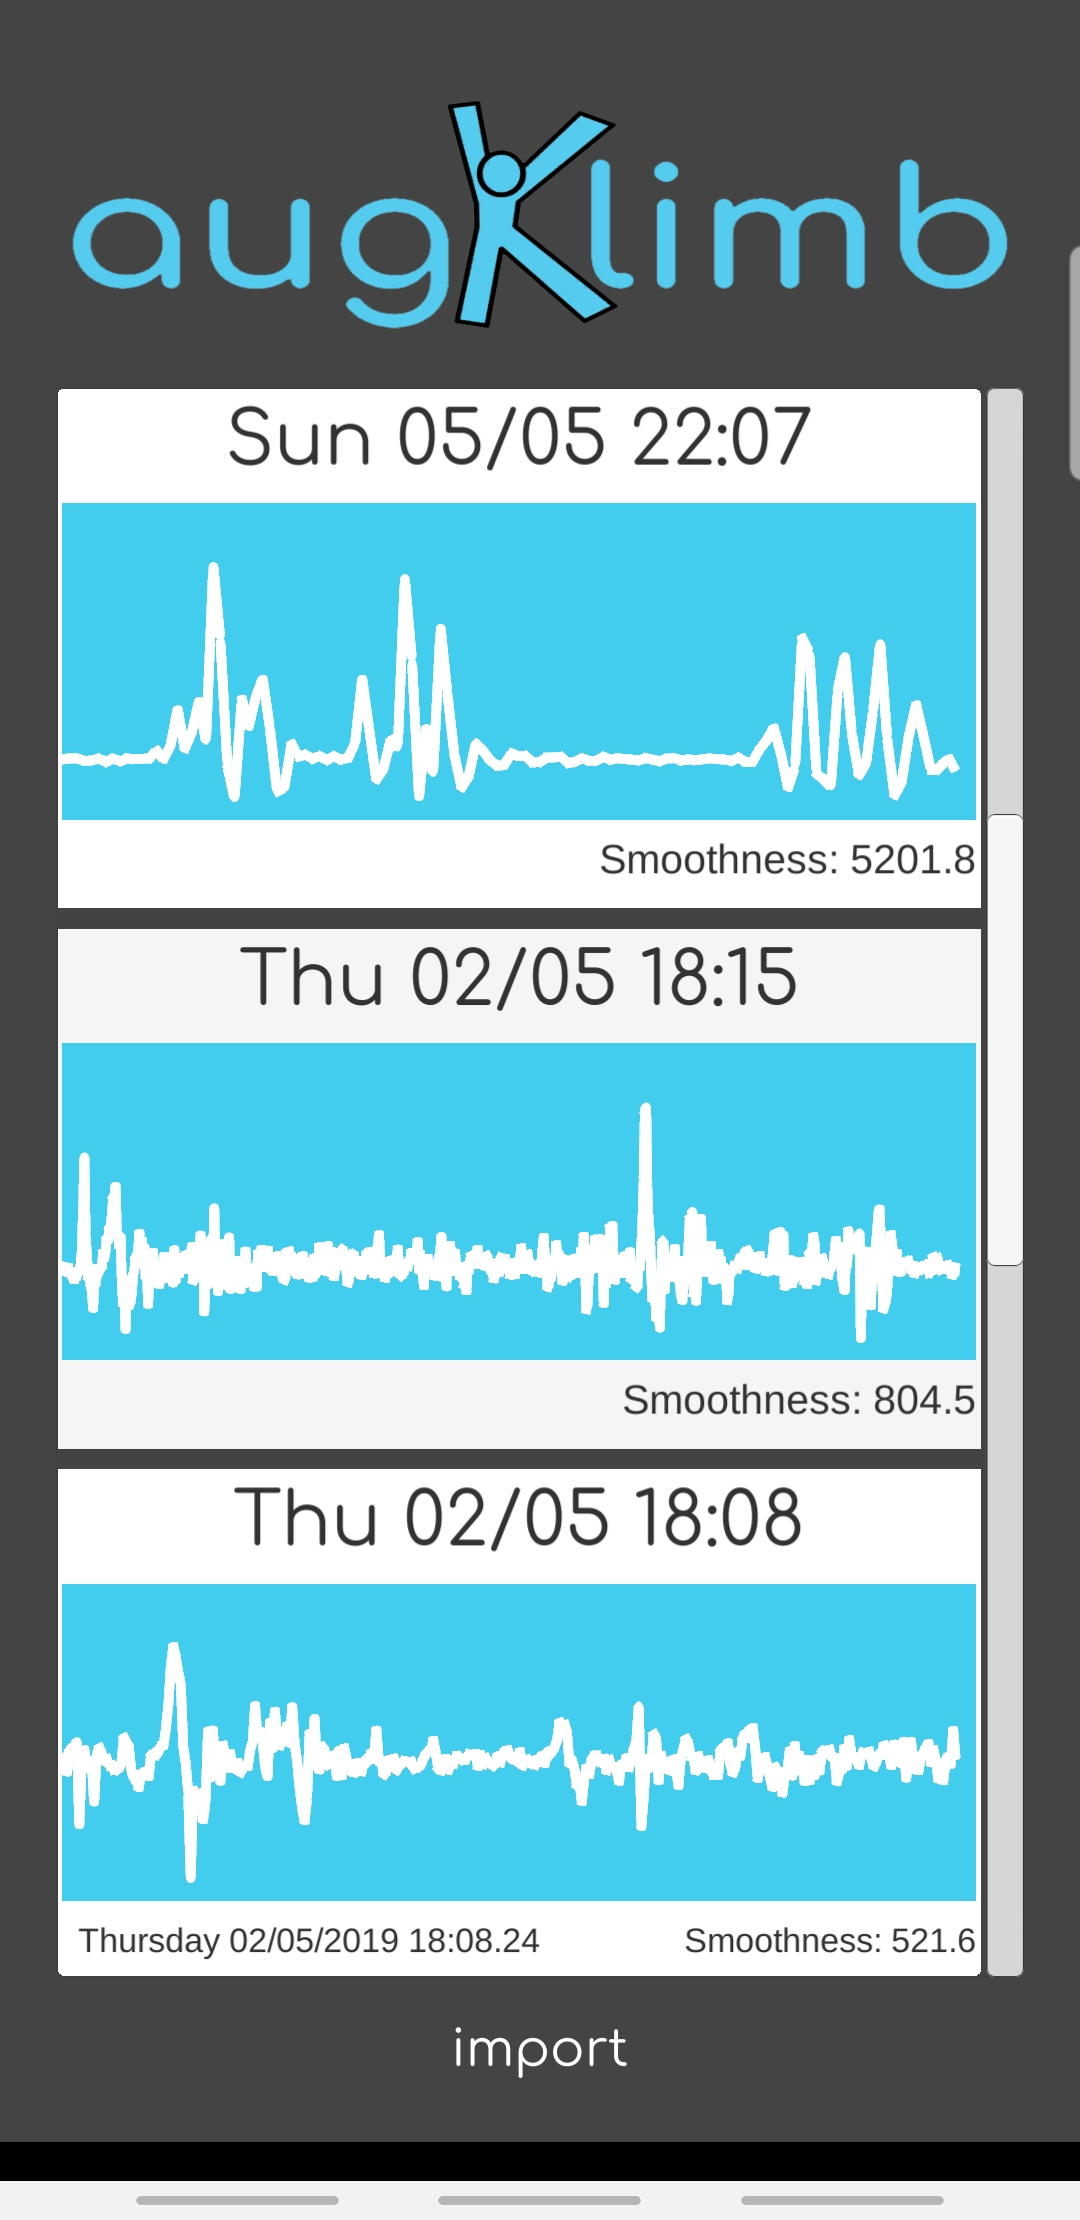
\includegraphics[width=6cm]{imgs/finalclimbview}
\caption{The final version of augKlimb's single-climb-viewing page}
\label{fig:finalclimbview}
\end{figure}




\subsection{Conflicting Requests From Users}
Due to the variety of use-cases the app can provide, a frequent side-effect of streamlining one user-flow was that other users would feed back that their preferred usage of the app had been hindered.

The biggest example of this was was which view to show the user upon completion of an accelerometer recording.
Some users who were using the graph to analyse their climbs, or wanted to quickly link a video recording, wanted that page to show up immediately after a recording had finished, rather than having to go back to view the lists of climbs and select that climb's page.
Others, who were just using the smoothness-score, only wanted to view that metric before being able to swiftly press the Record button again and continue climbing, and favoured the clean and simple UI that mode of operation provided, only occasionally going to look at the graphs to inspect weaknesses.

Differing proposals for improvements from both groups initially caused me to alter the app in each direction in turn, only when revisiting my changelog later did I notice that on a weekly basis I was switching back and forth between a very simplistic  UI and one that provided a lot of data, just dependant upon whose feedback I had been exposed to on those development and testing days.
To solve this, I invited three testers who fell across the above range, and prompted a discussion between them around both what they would expect to see, and what they wanted to see.
A compromise was formed, where the initial recording page showed nothing but the time elapsed and the smoothness score (see Figure~\ref{finalrecorderview}), with a shortcut link to that climb's specific page, which could contain the full list of statistics, graphs, editing abilities and video-linking facilities.



\begin{figure}[h]
\centering
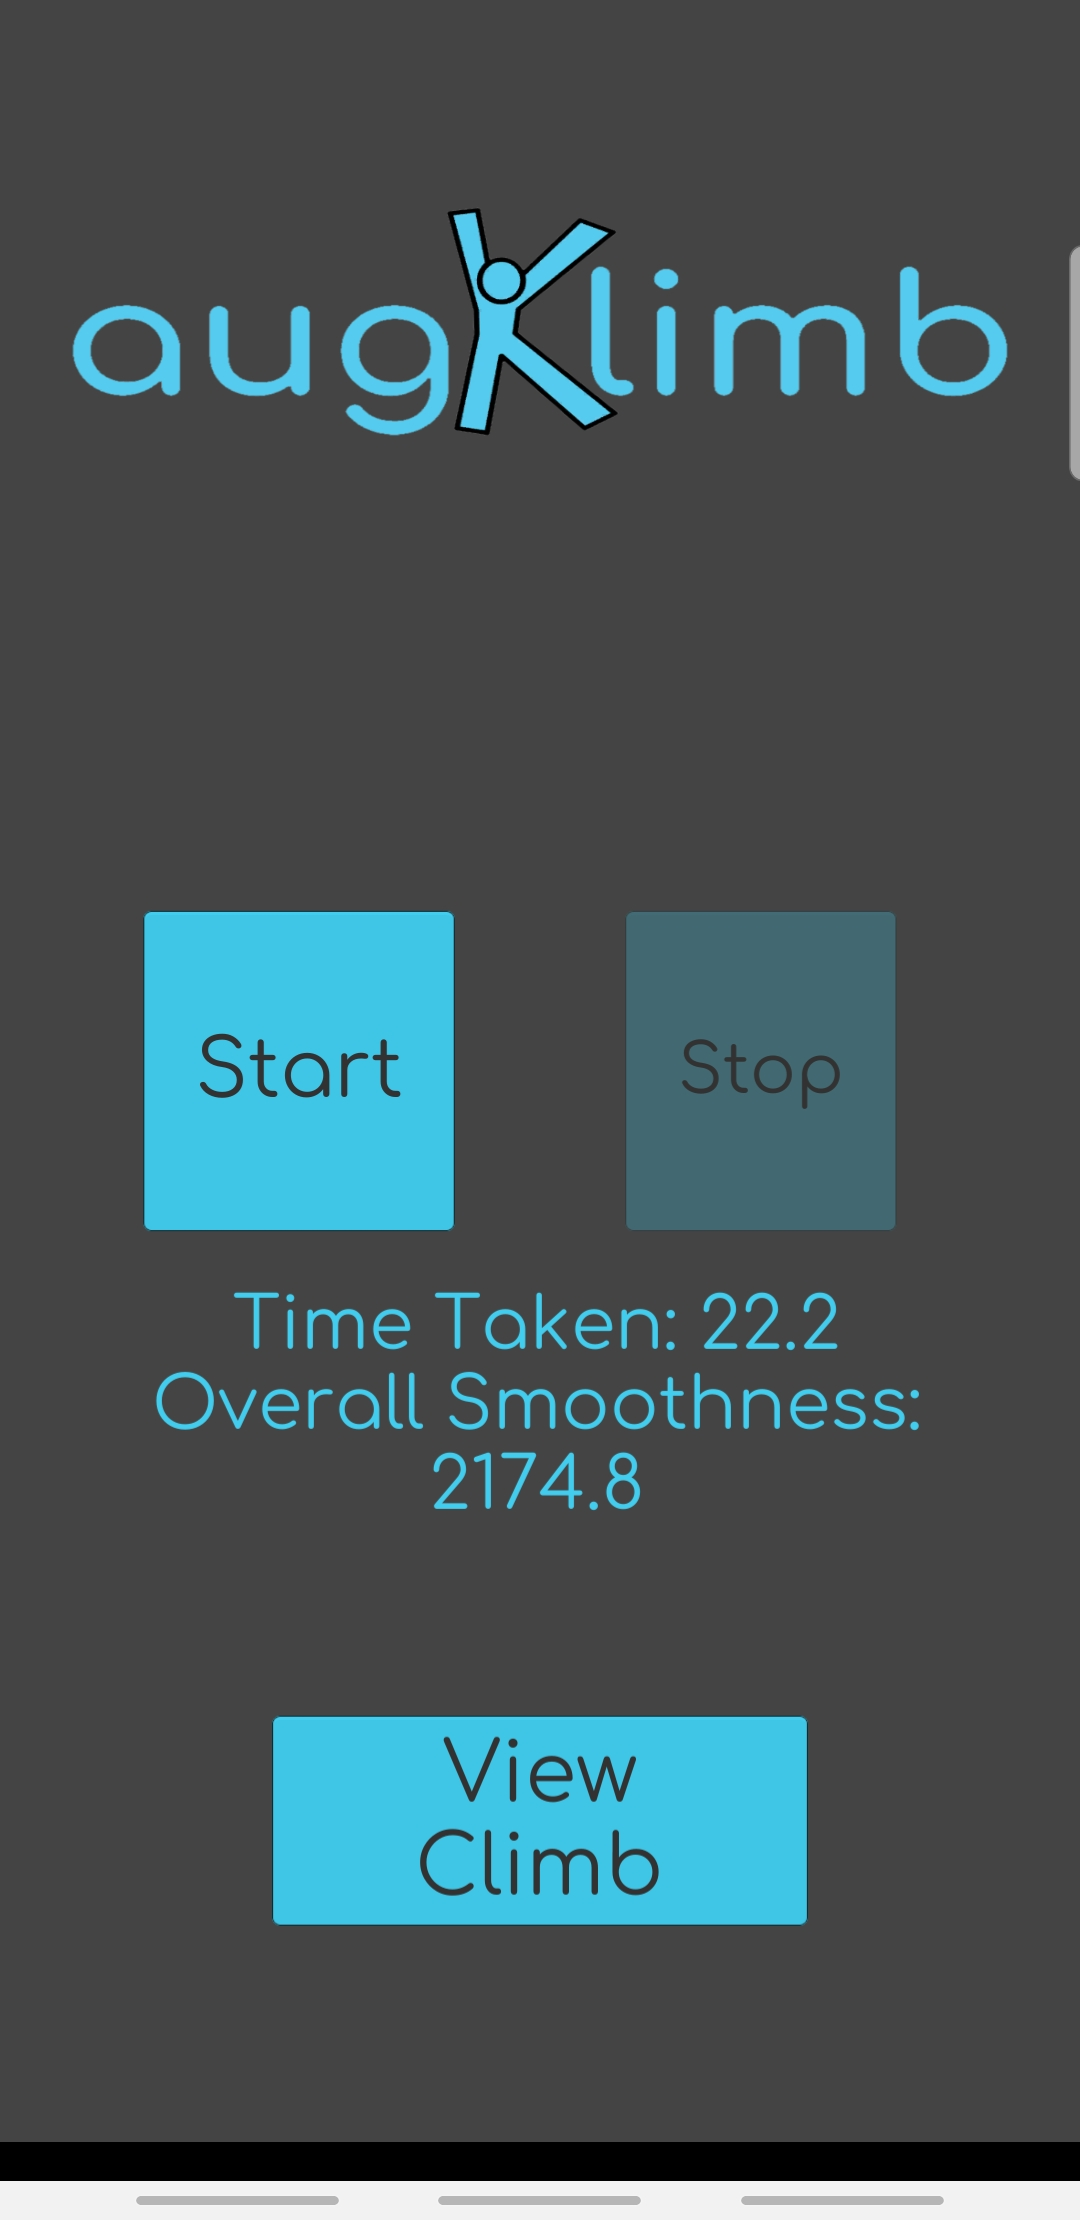
\includegraphics[width=6cm]{imgs/finalrecorderview}
\caption{The final version of augKlimb's post-recording view}
\label{fig:finalrecorderview}
\end{figure}


